\section{Developing robotic software with DUA}
\label{sec:dua_modules}
With the introduction of the \texttt{dua-utils} software collection in \Cref{sec:dua-utils}, the description of the Distributed Unified Architecture implementation and features is complete. Before discussing some results that led to its development, it is instrumental to see this framework in action. This section presents two software modules that are some of the most representative of the issues that DUA aims to solve, as well as of the functionalities that it provides to the developer to tackle them. Their choice is also motivated by the fact that they have been successfully employed in real-world scenarios during the course of this work, some of which are described in the following sections. In both cases, the aim is mainly to show how the DUA framework has been used to develop them and solve the integration issues that they presented; thus, an introductory description of their purpose and functionalities is given, followed by an explanation of how they have been configured as DUA units.

\subsection{Autonomous flight: flight\_stack}
\label{sec:dua_modules_flight_stack}
This project is a collection of software modules for autonomous drone flight and low-level control interfacing. The term \emph{autonomous drone}, in this context, identifies a flying robot: its structure can either be that of a multicopter, or a fixed-wing aircraft, or anything in between that flies, but it has no human operator for most of its operating time. Instead, the flight control and stabilization as well as planning tasks are entirely handled by onboard electronics, \emph{i.e.}, integrated computers and microcontrollers. The drone is supposed to be equipped with sensors of various kinds, such as inertial measurement units (IMUs), global navigation satellite systems (GNSS), LiDARs, and cameras, and actuators such as servos and motors.

Among the many kinds of autonomous robots, drones are one of the most difficult to develop and operate. This is due to their nature, which requires them to operate in three-dimensional space, and to the fact that they are used in scenarios where the environment may not be entirely known. The greatest complexity is due to the fact that drones are unstable systems, which means that they require continuous control to remain in the air and to perform the tasks they are assigned. Such control is usually achieved by means of a control loop that reads sensor data, computes the necessary corrections to the drone's attitude and position, and sends commands to the actuators in the form of torques and thrusts. The control loop runs at a frequency usually in the order of hundreds of Hertz, to ensure that the drone remains stable and responsive to external disturbances; for this to work, the most important source of feedback for an autonomous drone is the IMU, which provides the drone's attitude and angular velocity at a frequency that can get as high as \SI{1}{\kilo\hertz}. This tight timing requirement implies that basic flight stabilization and control is handled by a dedicated microcontroller, on which it runs as a task of some real-time operating system (RTOS) that ensures that the control loop runs at the required frequency.

The Pixhawk project \cite{meier_pixhawk_2011,meier_pixhawk_2012} represents a significant advancement in open-source flight control systems, establishing comprehensive hardware and software standards for autonomous aerial vehicles. The project implements a modular hardware architecture that supports multiple communication protocols and enables seamless integration of diverse sensors and actuators. This hardware framework operates in conjunction with the PX4 firmware \cite{meier_px4_2015}, an open-source flight control software developed at ETH Zurich and subsequently expanded under the Dronecode project \cite{dronecode_foundation_dronecode_nodate}. PX4 provides a modular control architecture that incorporates autonomous navigation, sensor fusion, and failsafe mechanisms, making it suitable for applications ranging from hobbyist projects to industrial systems. The combination of Pixhawk hardware standards and PX4 firmware capabilities creates a robust ecosystem that supports diverse autonomous operations, including agricultural monitoring, environmental data collection, and search and rescue missions. The system architecture emphasizes modularity, allowing individual components to be enabled or disabled based on mission requirements while maintaining efficient operation on resource-constrained hardware. Through sophisticated attitude estimation, position control, and advanced sensor fusion algorithms, this integrated platform delivers reliable state estimation even in challenging environments, establishing itself as a leading solution in both research and industrial applications.

Even if PX4 has evolved into a very powerful and flexible platform, there are some tasks that are still beyond its capabilities. To correctly perform its main task of basic flight stabilization, it has to remain a real-time software that runs on dedicated hardware. This means that it cannot be used to perform high-level tasks that require more computational power, such as computer vision, path planning, or decision-making. This is why the most recent control architectures for autonomous drones usually include a \emph{companion computer}, \emph{i.e.}, an SBC that runs a full operating system and that is connected to the flight controller through a serial or Ethernet link. The companion computer is responsible for all the high-level tasks that the drone performs, and it communicates with the flight controller to send to it the necessary commands. This way, the drone can perform sophisticated operations such as autonomous navigation, obstacle avoidance, or target tracking, while still being able to fly and stabilize itself thanks to the flight controller. This situation is depicted in \Cref{fig:ldc21hwarch}.
\begin{figure}[t!]
  \centering
  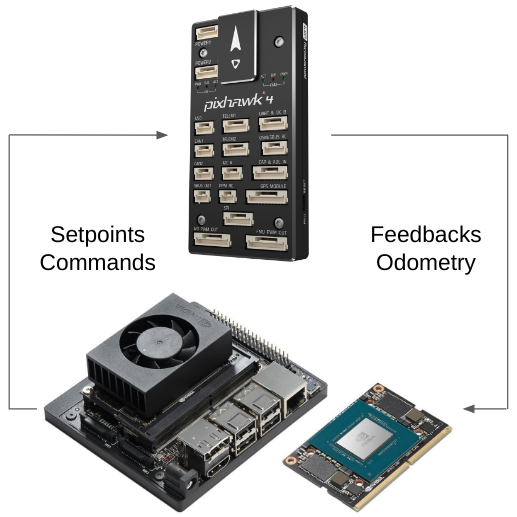
\includegraphics[width=.5\textwidth]{images/ch5/ldc21_hwarch.png}
  \caption{Functional diagram of a hardware architecture for autonomous flight: a Pixhawk 4 flight management unit (FMU) (top), and an Nvidia Jetson Xavier NX SBC (bottom).}
  \label{fig:ldc21hwarch}
\end{figure}

The flight management unit (FMU) is usually capable of passing all the necessary data to the companion computer, such as the drone's attitude, position, and velocity, as well as the status of the sensors and the actuators. The companion computer can then use this data to perform its tasks and send the commands back to the FMU. From the point of view of the companion computer, the drone is essentially the FMU: there is no distinction, since all the actuation and sensing technicalities are addressed by the FMU. Recalling the introductory discussion made in \Cref{sec:prb_design_challenges}, since an autonomous drone can be viewed as an autonomous robot, it is reasonable to suppose that its software architecture still follows a hierarchical organization. The FMU offers just a set of communication channels over which data can be sent but all of the technicalities involved in parsing this data, or sending the right commands and correctly parsing their feedback to request even a simple operation remain unsolved. Demanding this task to every single software module in the higher levels of the drone's control architecture leads to a seriously flawed design, just for a simple issue: if every module can talk to the FMU at the same time, who is actually controlling the drone at any given time? It appears clear at this point that, in such a sophisticated system, an entire layer of the architecture is reserved to modules that are in charge of interfacing with the FMU, abstracting the complexities of the communication protocols and the data formats, and providing a clear and consistent interface to the higher-level modules while handling all the necessary synchronization and arbitration tasks. This is the role of the \texttt{flight\_stack} \cite{masocco_flight_stack_nodate} DUA unit, which offers these functionalities thanks to the \ROS middleware and the PX4 firmware. Currently, it supports only multicopters but support for different types of aircraft is an ongoing development, and is based on version 1.13.3 of PX4. The \texttt{flight\_stack} repository contains five \ROS packages, the main three of which are called \texttt{px4\_msgs}, \texttt{micrortps\_agent}, and \texttt{flight\_control}.

The \texttt{px4\_msgs} package comes first since it contains a set of message definitions that are used to communicate with the FMU in both directions. These definitions correspond both in terms of fields and data types with the data packets that the modules of the PX4 firmware exchange internally among themselves. Thanks to this similarity, a module of the PX4 firmware easily serializes and deserializes packets coming from a serial UART link that connects the FMU with the companion computer. This module is called the \texttt{micrortps\_client}, and it is one of the real-time tasks of PX4; its peculiarity is that it follows the same real-time data transmission protocol that is implemented as part of the DDS standard presented in \Cref{sec:dds}. The other end of this communication is a task that runs on the companion computer, implemented as a \ROS node in the \texttt{micrortps\_agent} package. The operational task that this node performs is that of managing the serial interface connected to the FMU and interfacing it with the \ROS domain. For every different function of the PX4 firmware, there is a dedicated pair of message type and \ROS topic that the FMU either publishes or subscribes to. To make this possible, the \texttt{micrortps\_agent} node publishes or subscribes to the same \ROS topics that it offers as communication interfaces towards the FMU to other \ROS nodes running on the companion computer, handling FMU data serialization and deserialization as well as managing the serial UART link. To efficiently interface itself with the physical layer, as well as with \ROS, the \texttt{micrortps\_agent} makes use of both \ROS RMW and bare DDS APIs at the same time, the latter of which are provided by the eProsima Fast DDS implementation \cite{eprosima_fast_nodate}.

Having available a set of \ROS topics that expose all the functionalities of the PX4 firmware solves only the first half of the problem: abstracting the serial communication link and its technicalities, like message queueing and flow control, and translating it into a set of publish-subscribe communication primitives. What remains to be addressed is the abstraction of the whole drone, offering to the higher layers of the control architecture only a set of communication primitives which may even be more sophisticated than simple message topics but still hides a lot of complications concerning the execution of elementary tasks that the drone performs such as, \emph{e.g.}, takeoff and movement. This is the purpose of the \texttt{flight\_control} package, which is the core of the \texttt{flight\_stack} DUA unit.

In the control architecture of an autonomous drone, the \texttt{flight\_control} node is the first one that does not directly interface any hardware: to it, thanks to the first abstraction provided by the \texttt{micrortps\_agent}, the drone appears as another node in the architecture that communicates over a set of topics. The first, basic functionalities that the \texttt{flight\_control} offers are in fact based on this communication primitive: other nodes are expected to exchange data directly with the \texttt{flight\_control} using standard formats and it then translates the data into formats that PX4 expects and forwards the packets to the \texttt{micrortps\_agent}, which is in charge of sending them to the FMU on the serial link. Such first basic functionalities, all implemented with topics, include the following.
\begin{itemize}
  \item Position control, which is implemented by forwarding local position setpoints to PX4: nodes can send a setpoint in the form of a \ROS message, and the \texttt{flight\_control} translates it into a PX4 message and forward it to the FMU; note that this is also how hovering of a multicopter is achieved, since the \texttt{flight\_control} retains and republishes the most recent position setpoint at a frequency that avoids triggering PX4 failsafes.
  \item Velocity control, which is implemented by forwarding twist setpoints in body frame to PX4.
  \item Local pose data forwarding, for navigation in GNSS-denied environments or when an additional source of local position and orientation data is available and provided to PX4. This data has first to be transformed in a NED (North-East-Down) frame and then forwarded to PX4.
  \item PX4 local pose estimate republishing.
  \item Battery monitoring.
  \item PX4 log message monitoring.
\end{itemize}
More sophisticated functions are implemented using services and actions, that other nodes in the architecture can call acting as clients to request them and wait for their completion, receiving feedbacks in the meantime. These functions include the following.
\begin{itemize}
  \item Arming.
  \item Disarming.
  \item Takeoff.
  \item Landing.
  \item Basic movement to a specific position.
  \item Turn to a desired heading at the current position.
  \item FMU reboot.
\end{itemize}
For each of these functions, the \texttt{flight\_control} action and service servers exchange data with specific topics handled by the \texttt{micrortps\_agent}, gathering feedback and handling all possible outcomes and error conditions. In addition, the \texttt{fligth\_control} node also internally keeps track of the current operational state of the drone to allow every client to request only the operations that are possible in the current state. The \texttt{flight\_control} node is also in charge of handling the synchronization of the requests that it receives, to avoid that multiple clients request conflicting operations at the same time, and to ensure that the drone is always in a consistent state.

The relevant portion of the \texttt{flight\_stack} within the context of this work is its configuration as a DUA unit. It currently supports, and has been tested with, multiple targets ranging from SBC ones such as \texttt{jetson5}, to development ones such as \texttt{x86-cudev}. The unit configuration section of the Dockerfile for the \texttt{jetson5} target, intended for Nvidia Jetson SBCs presented in \Cref{sec:dua_supported_platforms_sbc}, is shown in \Cref{lst:flightstack}. Since no firmware development is performed on the SBC, the only configurations required concern the dependencies that are necessary for the \texttt{micrortps\_agent} to work. These include some Python packages, as well as an installation of the Fast-DDS-Gen tool by eProsima \cite{eprosima_fast-dds-gen_nodate}: this is required to generate IDL files that define messages for both the ROS and the serial side of the communications that the \texttt{micrortps\_agent} handles.

Development targets add to the aforementioned dependencies additional setup steps that configure what is required to build the PX4 firmware. For reference, \Cref{lst:flightstackdev} in \Cref{app:units} reports the unit configuration of the \texttt{x86-cudev} target. More dependencies are installed which are necessary to build the NuttX RTOS \cite{apache_software_foundation_apache_nodate}, which is the preferred real-time operating system to run the PX4 firmware on Pixhawk boards. Furthermore, since a cross-compiler is required to build the firmware in an x86 environment, version 9 of GCC \cite{free_software_foundation_gcc_nodate} for ARM is downloaded and decompressed. Finally, version 2.10.1 of eProsima Fast DDS and its dependencies are downloaded and built from source, to provide support for the compilation of the PX4-side of the communication protocol that the \texttt{micrortps\_agent} handles.

The \texttt{flight\_stack} DUA unit is a clear example of how DUA can be used to solve the integration issues that arise when developing software for autonomous systems. Focusing on the development targets, the initial dependencies are easily installed since they are distributed as packages for the system package manager and thus may be made part of the host system installation. The latter tools, however, are built from source and then installed system-wide, a process that may only be scripted at best. In contrast, DUA automates these integration and setup steps in a way that is transparent to the developer who, to use this unit, only needs to add it configuring their project targets as described in \Cref{sec:dua_template_configuration}.

\begin{center}
\begin{minipage}[t]{.9\textwidth}
\begin{lstlisting}[caption={Unit configuration of the \texttt{jetson5} target of the \texttt{flight\_stack} DUA unit \cite{masocco_flight_stack_nodate} as of November 26, 2024.}, label={lst:flightstack}]
# flight_stack START #
# Install PX4 general dependencies required by microRTPS Bridge
RUN apt-get update && apt-get install -y --no-install-recommends \
  astyle \
  libxml2-dev \
  libgstreamer-plugins-base1.0-dev \
  rsync && \
  rm -rf /var/lib/apt/lists/* /tmp/* /var/tmp/*/apt/lists/*

# Install PX4 Python dependencies required by microRTPS Bridge
RUN . /opt/dua-venv/bin/activate && yes | pip3 install -U \
  future \
  jinja2>=2.8 \
  jsonschema \
  kconfiglib \
  lxml \
  psutil \
  pygments \
  pymavlink \
  pyulog

# Build and install Fast-DDS-Gen (required by microRTPS Bridge)
WORKDIR /opt
RUN git clone --recursive --single-branch --branch 'v2.4.0' \
  https://github.com/eProsima/Fast-DDS-Gen.git && \
  cd Fast-DDS-Gen && \
  ./gradlew assemble && \
  ln -s /opt/Fast-DDS-Gen/scripts/fastddsgen scripts/fastrtpsgen && \
  cd .. && \
  chgrp -R internal Fast-DDS-Gen && \
  chmod -R g+rw Fast-DDS-Gen
WORKDIR /root
ENV PATH=/opt/Fast-DDS-Gen/scripts:${PATH}
# flight_stack END #
\end{lstlisting}
\end{minipage}
\end{center}

\subsection{Driving a sensor: zed\_drivers}
\label{sec:dua_modules_zed_drivers}
One of the hardest problems that autonomous robots face is that of localization: determining continuously its position and orientation (\emph{i.e.}, its \emph{pose}) within the environment. Robots are equipped with sensors, whose variety ranges from inertial measurement units to cameras, LiDARs, and GNSS receivers. These devices provide data that can later be used, either directly or by appropriate post-processing algorithms, to obtain an estimate of the current pose of the robot. The most common approach is that of sensor fusion, which consists of combining the data from multiple sensors to obtain an estimate of the robot's pose.

Among the many classes of sensors, RGB (Red-Green-Blue) cameras are one of the most versatile and widely used in robotics. They can range from cheap and lightweight solutions including, \emph{e.g.}, a single optic and producing only a video stream, to more expensive but sophisticated ones that include more optics and can provide additional information, such as depth maps. One of the most famous series of cameras aimed at robotics applications is the ZED series by Stereolabs \cite{stereolabs_stereolabs_nodate}. The ZED cameras are stereoscopic cameras, \emph{i.e.}, they mimic the human eye by housing two identical optics that are separated by a fixed, known distance. The sensors on each optic are synchronized, thus the frames they produce can be used to compute a depth map of the scene that the camera is viewing. This depth map can be expressed in a variety of formats, from grayscale images to point clouds, and can be employed in a variety of contexts, from obstacle avoidance to 3D environment mapping. ZED cameras have emerged as a solution also due to their software support offered by Stereolabs: the ZED SDK \cite{stereolabs_zed_nodate}. It is a versatile software development kit that enables programmers to easily interface with a ZED camera and get its data. One of the most famous disadvantages of working with images in real-time is the high cost in terms of computational power that is demanded to the host system: processing pictures usually requires a lot of memory and CPU power, and the more complex is the processing, the more resources are needed. The ZED SDK, however, has been designed to take advantage of Nvidia GPU devices present on the host, being it either a desktop computer or an SBC: thanks to the CUDA parallel computing platform, the internal algorithms of the ZED SDK can run in real-time and produce high-quality results even on low-power SBCs and similar devices. Thanks to this feature, the ZED SDK integrates a positional tracking module that, if activated, provides a real-time estimate of the pose of the camera in the environment, with respect to a reference frame that is placed at the camera's starting position. This estimate is obtained internally by the SDK algorithms by fusing the data from the camera's optics and the IMU.

In the context of a robotic software architecture based on \ROS, the integration of a sensor like a ZED camera requires the development of a specific module that abstracts it and publishes its data to the ROS network in standard formats. Such a module is usually called, in the ROS world, a \emph{driver node}: note that it is not a device driver but rather a software module that interfaces with a device and exposes its functionalities to the rest of the software architecture. It is called \emph{driver} because its task is that of of making the device work and of providing a clear and consistent interface to the rest of the nodes in the architecture, who should not be concerned with the technicalities of the device itself. The code of the driver node is based on the SDK of the device itself, if any, which is the ZED SDK in the case of the package discussed in this section: the \texttt{zed\_drivers} package \cite{masocco_zed_drivers_nodate}.

Like the other software modules discussed so far, \texttt{zed\_drivers} is a DUA unit that contains multiple \ROS software packages. The main package is called \texttt{zed\_driver} and it is the subject of the current discussion. To briefly introduce it, consider first the task that the corresponding node has to perform: a ZED camera is a hardware device that must first be opened, specifying a set of configuration parameters for its various functions, then started, and finally its data may be read, processed, and published to the \ROS network. This is, in essence, a summary of the structure of the \texttt{zed\_driver} node implemented by the package.

At startup, the \ROS node parses its parameters: these specify many configuration options of the supported functionalities of the camera, ranging from resolution and framerate, to depth sensing mode and depth map size, to IMU sampling rate. The node then initializes the ZED camera, setting it up according to the options that the parameters specified, and starts it. The node then enters a loop where it reads the data produced by the camera. The data can be divided in four main categories: RGB frames, depth maps, positional tracking data, and IMU samples. Each of these four sets of data has to be processed before it can be published over the \ROS network, mainly because it has to be copied from the program memory to properly-formatted \ROS messages that encode standard sensor data types. To streamline execution, the \texttt{zed\_driver} node runs four parallel threads that handle each type of data separately at the same time, optimizing the use of system resources to reduce latencies and ensure that the data is published before the camera produces the next frames, so that the node can keep up with the camera's framerate; the IMU thread, in particular, runs at a higher frequency sampling the camera IMU independently of the optics, since it runs at a higher rate. RGB frames have to be converted to \ROS image messages, depth maps to point cloud messages, positional tracking data to pose messages and transformations, and IMU samples to IMU messages. The node then publishes these messages over appropriate topics.

To summarize the node's capabilities, here are the ZED SDK functionalities that it supports, each with a complete set of configuration options exposed as node parameters.
\begin{itemize}
  \item RGB video stream.
  \item Depth maps and point clouds computation.
  \item IMU sampling.
  \item Pose estimation with the positional tracking module.
  \item Raw camera data logging in SVO files.
  \item Real-time video stream over the network with NVENC encoding \cite{nvidia_nvidia_nodate-1}.
\end{itemize}
To achieve this, the code of the node makes wide use of the ZED SDK C++ API. Coming back to the scope of this work, this means that a compatible installation of the ZED SDK has to be present on the host system to which the camera is connected. According to the official documentation, setting it up is easy since it is distributed as a script that first installs the dependencies and then the SDK itself. The system on which the script is run has to meet a certain set of requirements: it has to be a Ubuntu \cite{canonical_ubuntu_nodate} system with some dependencies already in place and it must have a Nvidia GPU with a version of the CUDA toolkit \cite{nvidia_cuda_nodate-1} installed which is also compatible with the version of the ZED SDK that one is installing. In the case of Jetson SBCs, things get more complicated because additional libraries, distributed by Nvidia via the JetPack SDK installation, are required. The \texttt{zed\_drivers} DUA unit automates all these setup steps, making the installation of the ZED SDK and the configuration of the project repository a matter of minutes.

Before delving into two example unit configuration Dockerfiles, recall that the system environments offered by DUA base units are stable and configured in a way to offer a good set of system packages that are ensured to be compatible with each other. Still, to install an SDK that is distributed as a self-installing script, one has to do some level of work on each target to ensure that the installation runs smoothly in a reproducible way and that it actually results in a usable SDK.

The \texttt{zed\_drivers} unit supports only targets aimed at systems that may have an Nvidia GPU. \Cref{lst:zeddriversjetson5} shows the unit configuration for the \texttt{jetson5} target. In this case, the setup is pretty straightforward: after an initial set of system dependencies that the SDK installer necessarily expects, the ZED SDK installation script is downloaded and executed. Note that, due to a compatibility issue with an Nvidia library, the version that is downloaded supports a higher JetPack version than the one on which the base unit is based: this is one of the many kinds of integration issues that usually happen in this field and that, to be solved, might require many reinstallation or board reflashes. The DUA framework, on the other hand, grants the developer the possibility to make many quick subsequent attempts without the need to reflash the Jetson board each time, by simply modifying the Dockerfile and rebuilding the image. The only critical configuration step is then the creation of a fake \texttt{/etc/nv\_tegra\_release} file that the SDK installer expects to find to correctly identify the system on which it is running, which apperas to be missing in Nvidia JetPack Docker images.

The unit configuration for the \texttt{x86-cudev} target is shown in \Cref{lst:zeddriversx86cudev}: surprisingly, this is more intricate than the one for the Jetson boards. First, due to other incompatibilities with the contents of the official Nvidia image, cuDNN \cite{nvidia_cuda_nodate} and cuBLAS libraries have to be upgraded to the latest version, the latter of which even requires a manual installation from the contents of its system package. Then, finally, the ZED SDK can be installed by downloading its installer script and running it, requiring no additional steps.

At the end of this section, after these units have been discussed as examples of how the DUA framework can help solve integration issues and provide replicable and reliable development environments, it is possible to note that thanks to the contents of these units a working prototype of an autonomous system such as an autonomous drone can be set up in a matter of minutes: first, a DUA project has to be created, adding the units to it and configuring supported targets as illustrated in \Cref{sec:dua_template_configuration}. Then, the project can be deployed onto a compatible SBC to be installed on the prototype and what is left to be done is just to download the base unit image and build the target image on top of it. A development image is then also set up to build and flash the microcontroller firmware. The necessary software modules are then ready to be built, configured, and run on the SBC, and the prototype may be tested right away.

\begin{center}
\begin{minipage}[t]{.9\textwidth}
\begin{lstlisting}[caption={Unit configuration of the \texttt{jetson5} target of the \texttt{zed\_drivers} DUA unit \cite{masocco_zed_drivers_nodate} as of November 26, 2024.}, label={lst:zeddriversjetson5}]
# zed_drivers START #
# Install ZED SDK dependencies
# (Nvidia stuff should already be installed in the base unit)
RUN apt-get update && \
  apt-get install -y --no-install-recommends \
  apt-transport-https \
  udev \
  zstd && \
  rm -rf /var/lib/apt/lists/* /tmp/* /var/tmp/*/apt/lists/*

# Install the ZED SDK
# We currently support version 4.1
# Do some more black magic here to enable streaming features
# on Jetson inside a container.
# The syntax for the echo is:
# R${L4T_MAJOR_VERSION} (release), \
#   REVISION: ${L4T_MINOR_VERSION}.${L4T_PATCH_VERSION}
# NOTE: We install an SDK version for a newer version of JetPack
# than that of this base image, due to an incompatibility with the
# deprecated libnvbuf.
RUN echo "# R35 (release), REVISION: 2.1" > /etc/nv_tegra_release && \
  wget --no-check-certificate -nc -O zed_sdk.run \
  https://download.stereolabs.com/zedsdk/4.1/l4t35.4/jetsons && \
  chmod +x zed_sdk.run && \
  ./zed_sdk.run -- silent skip_python && \
  rm zed_sdk.run && \
  ln -sf /usr/lib/aarch64-linux-gnu/tegra/libv4l2.so.0 \
  /usr/lib/aarch64-linux-gnu/libv4l2.so && \
  rm -rf /var/lib/apt/lists/* /tmp/* /var/tmp/*/apt/lists/* && \
  chgrp -R internal /usr/local/zed && \
  chmod -R g+rwx /usr/local/zed
ENV LD_LIBRARY_PATH=${LD_LIBRARY_PATH}:/usr/local/zed/lib
ENV LOGNAME=neo
# zed_drivers END #
\end{lstlisting}
\end{minipage}
\end{center}

\begin{center}
\begin{minipage}[t]{.9\textwidth}
\begin{lstlisting}[caption={Unit configuration of the \texttt{x86-cudev} target of the \texttt{zed\_drivers} DUA unit \cite{masocco_zed_drivers_nodate} as of November 26, 2024.}, label={lst:zeddriversx86cudev}]
# zed_drivers START #
# Install ZED SDK dependencies
# NOTE: Here we require an upgrade to make sure
# we have the latest Nvidia libraries.
RUN apt-get update && apt-get install -y \
  --no-install-recommends --allow-change-held-packages \
  libcudnn8 \
  libcudnn8-dev \
  zstd && \
  rm -rf /var/lib/apt/lists/* /tmp/* /var/tmp/*/apt/lists/*

# Install libcublas-12-0 libraries manually
# to fix some incompatibilities in ZED SDK dependencies
WORKDIR /tmp
RUN apt-get update && \
  apt-get download libcublas-12-0 && \
  mkdir contents && \
  dpkg-deb -xv libcublas-12-0_12.0.2.224-1_amd64.deb contents/ && \
  mv contents/usr/local/cuda-12.0/targets/x86_64-linux/lib/* \
  /usr/local/cuda/lib64/ && \
  rm -rf contents libcublas-12-0_12.0.2.224-1_amd64.deb && \
  ldconfig && \
  rm -rf /var/lib/apt/lists/* /tmp/* /var/tmp/*/apt/lists/*
WORKDIR /root

# Install the ZED SDK
# We currently support version 4.1
RUN wget -nc -O zed_sdk.run \
  https://download.stereolabs.com/zedsdk/4.1/cu118/ubuntu22 && \
  chmod +x zed_sdk.run && \
  ./zed_sdk.run -- silent skip_python && \
  rm zed_sdk.run && \
  rm -rf /var/lib/apt/lists/* /tmp/* /var/tmp/*/apt/lists/* && \
  chgrp -R internal /usr/local/zed && \
  chmod -R g+rwx /usr/local/zed
ENV LD_LIBRARY_PATH=${LD_LIBRARY_PATH}:/usr/local/zed/lib
# zed_drivers END #
\end{lstlisting}
\end{minipage}
\end{center}
